\setcounter{chapter}{2}

\chapter{Coalition Formation and Coopetitive Behavior of Autonomous Web Services}\label{sec:coalitionformationws}

In this chapter, we present our coalition model of agent-based web
services within communities \cite{SCC2013efficient}. We start by describing the general
architecture and considered parameters for web services.
Thereafter, problem modeling and formulation will be introduced in
terms of task distribution and community revenue. Web service
cooperative games in different settings will follow along with
some simulation results.

\section{Preliminaries}\label{s:preliminaries}

Our system consists of three main types of entities working
together: \emph{1) Web services} are rational entities that aim to maximize
their utilities by providing high quality services to end users.
They aim to maximize their individual income by receiving enough
requests from end users. In order to increase their revenue, web
services seek for more tasks if they have the capacity and
throughput to do so. Web services can join communities to have
better efficiency by collaborating with others, to have access to
higher market share, and to have opportunity of receiving a bigger
task pool from end users. Throughout this proposal, in our
equations, we refer to web services as $ws$ and to the set of web
services hosted by a given community as $C$.
%To simplify the
%notation, sometimes we simply write $ws$ instead of $ws \in C$ to
%go through the elements $ws$ of the set $C$.
\emph{2) Master Web Services} or the community coordinators, are representatives of the
communities of web services and responsible for their management.
Communities receive requests from users and aim to host a healthy
set of web services to perform the required tasks. They seek to
maximize user satisfaction by having tasks accomplished according
to the desired QoS.
%In fact, higher user satisfaction will bring
%more user requests and increase the market share and revenue of
%the community.
\emph{3) Users} generate requests and try to find the best
available services. User satisfaction is abstracted as function of
quantity and quality of tasks accomplished by a given service.
Higher user satisfaction leads to higher trust of the community by users hence directing more requests towards that service provider.

Web services come with different quality of service parameters.
These parameters include availability, reliability, successability, throughput, latency, capacity, cost, regulatory and security \cite{DBLP:conf/smc/Al-MasriM09a}\footnote[1]{The implemented environment includes the QWS dataset by Eyhab Al-Masri and Qusay H. Mahmoud freely available at: http://www.uoguelph.ca/\textasciitilde{}qmahmoud/qws/.}.
We adopted a real world dataset \cite{DBLP:conf/smc/Al-MasriM09a}
which has aggregated and normalized each of these parameters to a
real value between 0 and 1. Since requests are not shared among
web services and are distributed among all of them inside a
community, each one of them comes with a given QoS denoted by
$(QoS_{ws})$. We assume that $(QoS_{ws})$ is obtained by a certain linear weight function of the parameters. We use this quality output later in evaluating the
community \emph{worth} or \emph{payoff} function.

Figure 3 represents our revised architecture of web service
communities where tasks are to be distributed among the members
that are interested in forming stable coalitions. As discussed in
Chapter 2, communities are essentially virtual platforms
aggregating web services having similar and complementary
functionalities and communicate with other entities such as UDDI
registries and users using particular protocols. Web services join
communities to increase their utility by having larger market
share and task pool.
%Community coordinators or master web services
%are responsible for community development, managing membership
%requests from web services and distributing user tasks among the
%community members. Community coordinators try to attract quality
%web services and keep the community as stable and productive as
%possible to gain better reputation and user satisfaction, which
%results in having higher revenue.

\begin{figure*}[!t]
\centerline{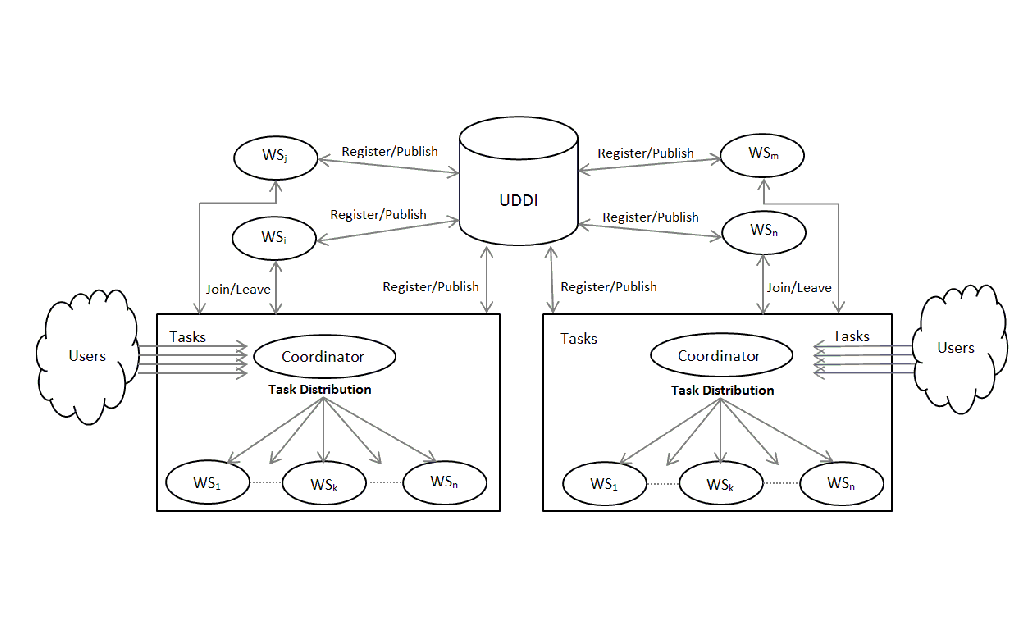
\includegraphics[width=15cm]{community.eps}}
\caption{Architecture of Web Service communities}
\label{fig_community}
\end{figure*}


\section{Problem Formulation and Modeling}\label{s:model}

In this section, we present  web services and community coordinator's interactions, the task distribution process and revenue models in web service communities.

\subsection{Task Distribution}

As mentioned in Section \ref{s:preliminaries}, communities
are robust service providers with well established market share
and reputation. By maintaining their reputation and performance,
they attract  end users which choose them as service providers to
perform their tasks. The community master is characterized by a
request rate $(R_C)$ from users. Each web service comes with a
given QoS ($QoS_{ws}$) from which the throughput $Th_{ws}$ is
excluded. Throughput is the average rate of tasks a web service
can perform per time unit. Its exclusion from $QoS_{ws}$ allows us
to build our analysis on the particular value of $Th_{ws}$. Thus,
web services perform tasks with an average output quality of
$QoS_{ws}$ and a throughput rate of $Th_{ws}$.

The community master uses a slightly modified \emph{weighted fair queuing} method to distribute tasks among its members. The goal is to allocate incoming tasks to web services with a rate matching the throughput value of $Th_{ws}$. In \emph{weighted fair queuing} method \emph{all} the input flow is multiplexed along different paths, however in our case if the input rate $(R_C)$ of the community is more than the summation of throughput values of the web services in the community, some of the input tasks will be queued and served with delay. Thus, the amount of tasks performed by community is $\sum_{ws \in C}{(Th_{ws})}$ when $\sum_{ws}{Th_{ws}} \leq R_{C}$. However, when the input rate $(R_C)$ of the community is less than the summation of throughput values of the web services in the community,
%the community has more web services having more total throughput value than community's request rate
$(R_C)$ the \emph{weighted fair queuing} algorithm assigns a weighted task rate of $R_C \times \frac{Th_{ws}}{\sum_{ws}{Th_{ws}}}$ for each web service ($ws$) and the total rate of tasks being performed is $R_C$, the community's receiving request rate.

While distributing tasks, the community master can verify the performance, throughput and quality of service of   tasks being performed by web services. It can recognize if web services are capable of doing the amount of tasks they advertised. If for any reason there is a decline in quality metrics or throughput, the  community master will announce the new parameters and community masters and members can consider those values as benchmark for future performance calculations. 
Web services that got their quality declined are penalized, and in this way, players have incentive to reveal their real capabilities to profit best from the community and to avoid being penalized. In addition, the system should be dynamic enough to detect and react to web services quality metrics variation as over time web service metrics may  degrade or improve, a change that the community should adjust to.
% Therefore its easy for the system to encourage players to be in some sense incentive compatible in the way that they would profit best by truthfully revealing their capabilities. Also it is important to be dynamic enough to consider web services which may have their quality metrics degraded or even improved over time for any reason and be able to adjust the community with new parameters.

\subsection{Community Revenue}

The communities and web services earn revenue by performing tasks.
The total gain is function of quality ($QoS_{ws}$) and throughput
($Th_{ws}$) of tasks being performed. We have adopted a linear equal weight average over
the QoS parameters excluding the
$Throughput$ and $Cost$ parameters. A community has the option to
weigh specific QoS parameters depending on the expectations of
their clients.

The maximum potential output of a community $(PO(C))$  is an aggregation of number of tasks, times their quality, for each web service member of the community:

\begin{equation}
PO(C) = \sum_{ws \in C}{(T_{ws} \times QoS_{ws})}
\end{equation}

If the summation of throughput values ($Th_{ws}$) of community members exceeds the input task rate of the community ($R_C$) the community cannot perform at its maximum potential. It denotes the case when the community has more web services than it needs to perform the input task load. The actual output has to be normalized to the amount of tasks being performed.

\begin{equation}\label{out_c}
Out(C) = \left\{
  \begin{array}{l l}
    PO(C) & \quad \text{if $\sum_{ws}{Th_{ws}} \leq R_{C}$}\\
    PO(C) \times \frac{R_{C}}{\sum_{ws}{Th_{ws}}} & \quad \text{if $\sum_{ws}{Th_{ws}} > R_{C}$}
  \end{array} \right.
\end{equation}

The revenue function of the web service community is a linear function of $Out(C)$ with a positive constant multiplier.


 \section{Web Service Cooperative Games}\label{s:game_solution}

In this section, we present different web service community models
and focus on the problem of how both web services and community
masters as rational entities would adopt strategies to maximize
their payoff.

\subsection {Web Services and One Community}

In this scenario, we assume the existence of a typical community
managed by its master, and web services need to join it to be able
to get requests from the master. The community master is
characterized by a requests rate $(R_{C})$ from users. Each web
service comes with a given QoS ($QoS_{ws}$). The worth of a community
$v(C)$ is set to Out(C) based on equation \ref{out_c}.

As mentioned in previous section, the worth and output of a
community  is a function of the
throughput and provided QoS of its web service members. If the throughput rate is more than
the master's input request rate, it means the web services inside
the community are capable of serving more requests than the
demand. Considering this factor, the valuation function is
designed to balance the output performance so that it matches the
exact throughput rate and QoS the web service can provide within
the particular community.
%** In the case where the limited tasks are distributed among web services uniformly, the value of coalition would be the proportion of the average QoS times their throughput to rate of available requests. **

In this first scenario, we only consider one grand coalition and
analyze the system from the point of view of one single master web
service and a collection of web services. The master web service
decides which members can join
%or should leave%
the community and distributes the requests and income among its
community members.

%\begin{figure}[!t]
%\centering
%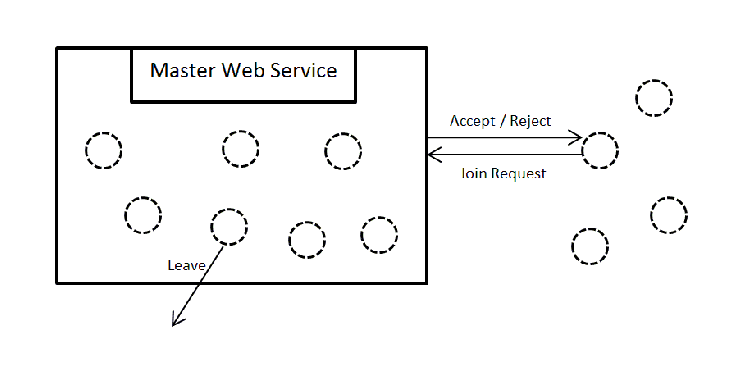
\includegraphics[width=3in]{Figures/s1.eps}`
%\caption{Web Services and A Grand Community}
%\label{fig_sim1}
%\end{figure}

The membership decision is made based on throughput and \emph{QoS}
of the considered web service. The goal is to have quality web
services in the community so it stays stable and no other web
services would have incentives to deviate and leave the coalition
$C$. Therefore, a basic method would be to check the core of the
coalition $C$ considering all the current community members (all
web services already residing within the community) and the new
web service. This algorithm uses the \emph{Shapley value}
distribution method as described in Equation \ref{eq:shapley} to
distribute the gain of $v(C)$ among all the members and then
checks if the \emph{Shapley value} payoff vector for this
community having the characteristic function $v(C)$ is in the
\emph{core}. In the \emph{Shapley value} payoff vector, the payoff
for each web service $ws_i$ is calculated based on its marginal
contribution $v(C \cup {i}) - v(C)$ over all the possible
different permutations in which the coalition can be formed, which
makes the payoff distribution fair. Because of going through all
the possible permutations of subsets of $N$, the nature of the
\emph{Shapley value} is combinatorial, which makes it impractical
to use as the size of our coalitions grows. However, it is proven
that in convex games, the \emph{Shapley value} lies in the core
\cite{DBLP:conf/ijcai/GrecoMPS11, myerson1991game}. Thus, if the
\emph{Core} is non-empty, the payoff vector is a member of the
\emph{Core}. The following proposition is important to make our
algorithm tractable.


\subsection {Web Services and Many Communities}

In this scenario, we consider multiple communities managed by
multiple master web services, each of which is providing
independent request pools. Identical
to the first scenario, master web services form coalitions with
web services. We use coalition structure formation methods to
partition web services into non-empty disjoint coalition
structures. The used
algorithms in \cite{Sandholm:1999:CSG:317145.317152,DBLP:conf/ijcai/GrecoMPS11,DBLP:conf/ijcai/RahwanMJ11} try to
solve key fundamental problems of what coalitions to form, and how
to divide the payoffs among the collaborators.

%\begin{figure}[!t]
%\centering
%\includegraphics[width=3in]{Figures/s2.eps}
%\caption{Web Services and Many Communities}
%\label{fig_sim2}
%\end{figure}

In coalition-formation games, formation of the coalitions is the
most important aspect. The solutions focus on maximizing the
social welfare. For any coalition structure $\pi$, let
$v_{cs}(\pi)$ denote the total worth $\sum_{C \in \pi}{v(C)}$,
which represents the \emph{social welfare}. The solution concepts
in this area deal with finding the maximum value for the social
welfare over all the possible coalition structures $\pi$. There
are $centralized$ algorithms for this end, but these approaches
are generally NP-complete. The reason is that the number of all
possible partitions of the set $N$ grows exponentially with the
number of players in $N$, and the centralized algorithms need to
iterate through all these partitions.
%These algorithms \cite{DBLP:conf/ijcai/GrecoMPS11, DBLP:conf/ijcai/RahwanMJ11, RePEc:wpa:wuwpga:0110001} are centralized algorithms, where all the complexity. However these algorithms are more intractable than Core stable solutions and practical with some constraints in practice\cite{RePEc:wpa:wuwpga:0110001}.
In our model, we propose using a distributed algorithm where each
community master and web service can be a decision maker and
decide for its own good. The aim is to find less complex and
distributed algorithms for forming web services coalitions
\cite{DBLP:journals/igtr/AptW09,Dieckmann02dynamiccoalition,ray2007game}.
The distributed merge-and-split algorithm in
\cite{DBLP:journals/igtr/AptW09} suits our application very well.
It keeps splitting and merging coalitions to partitions which are
preferred by all the players inside those coalitions.


\section{Taxation, Subsiding and Community Stability}\label{s:tax}

We discussed $core$ as one of the prominent solution concepts in
cooperative games. Working together, completing tasks and
generating revenue, agents need to distribute the gain in a way no
agents would gain more by forming their own group. However, in
most cases, the core of a game is empty, so we introduced the
\emph{$\epsilon$-core} concept, where agents would only earn a
minimal amount of $\epsilon$ by deviating from the coalition.
Stability is an attractive property for communities. In addition,
communities would benefit by having slightly more web services
than the exact number of web services needed to satisfy the task
rate cap. This is because there is always a possibility that the
web services may leave the community or they may under perform and
degrade the quality values they were initially performing with.

The solution we propose for communities to ensure stability is
applying a tax $\epsilon$, which is an amount of cost for those
web services that decide to change communities (let us say from
$C$ to $C'$), which would make deviation a costly act. However,
this would require all the community coordinators to agree on a
same amount of taxation, being governed by some external entities;
otherwise, web services would join communities charging the lowest
amount of tax. Before deciding to change the community, each web
service $i$ has to be sure that the gain $g_i(C \rightarrow C')$
calculated in Equation \ref{eq:gainsh} based on the Shapley values
of $i$ in the previous and new communities and the tax $\epsilon$
is positive, which means, what the web service would gain in $C'$
is greater than what it gains in $C$ and the tax it would pay if
moving all together:


\begin{equation}\label{eq:gainsh}
g_i(C \rightarrow C') = \phi_i(C',v) - \phi_i(C,v) - \epsilon
\end{equation}


Another viable solution we introduce to our scenario is to
stabilize the game using external subsidies. The reason a game is
not stable is that the community is not making enough revenue to
allocate enough gain to the players. A community coordinator can
subside its community with a constant coefficient value of
$\lambda$.
%
%Rewarding a community with high number of quality participants
%with $\lambda v(C)$, where $\lambda \leq 1$.
%
Obviously, with a big value for $\lambda$, it is always possible
to stabilize the community. However, this can be a costly act for
the community coordinators, so they are interested in the minimum
subside value of $\lambda$ making the community stable. This can
be achieved by solving the following linear program:
%
  \begin{alignat*}{3}
    \min~   & \lambda  \\
    \text{s.t. } & \lambda v(C) > v(C') & ~& \text{ for all } C' \subset C
  \end{alignat*}


%When a new web service $i$, wants to join the community, the
%valuation function of the community members and the new web
%service is subsided by the community coordinator in order to
%incentivize formation of this community and is set to:
%\begin{equation}\label{eq:taxv}
%v'(C \cup \{i\}) = \lambda \times v(C \cup \{i\})
%\end{equation}
%In equation \ref{eq:taxv} the value of $v'$ is
%replaced with the valuation function for the new forming coalition
%$C \cup \{i\}$.
Subsiding or taxing in order to reduce the
bargaining power of sub coalitions are called $taxation$
\cite{eps346856} methods. We evaluate the effectiveness of these
two methods experimentally through extensive implementations in
the next section.



%Thus, another way to garantee \emph{$\epsilon$-core} stability can be achieved by some surplus payments from community coordinators. These concepts of applying cost in coallition values in order to reduce their bargaining power are called $taxtation$ methods\cite{eps346856}.

%The \emph{$\epsilon$-core} concept, in its definition, considers the willing to join or deviate from agent's point of view. It claims agents for any reason will be not willing to deviate to gain less than $\epsilon$ amount of profit. Communities can agree on However, in our case, the community master is willing to keep web services in communities too. There are several reasons for this, one reason is there is always possibility that agents may leave the community or they may under perform from the quality values they were initially performing with. To this end, our communities will reward and valuate web services in the community

\section{Coopetitive Behavior of Services within Communities}\label{s:coop}

In previous sections, our focus was on community formation and we emphasised on cooperative behavior of the web services as agents. Within communities, those services, selfish and utility maximizers by nature, can follow two different strategies, namely cooperation and competition in order to increase their payoffs when they provide services to consumers \cite{VuFind-10008938119}. In typical business settings, services are used to compete within communities as they provide the same functionalities and the number of users requests is finite. However, the same reason of providing similar functionalities can lead services to cooperate because they can replace each other in case of failure or unavailability, and services can do better in a coalition structure. Analyzing services competition and cooperation strategies within communities is still an open problem that motivates the research described in this section. we propose a mechanism within which service agents
in the community could choose either to compete for an announced task\footnote{Requests and tasks are used in this report interchangeably.}, or to cooperate with other competing services in the same community to accomplish some subtasks of the announced task. We equip intelligent web services to follow a reasoning technique to choose best interactive strategy (Coopetitive attitude, which is categorized to compete and cooperate). In the proposed system, We explore details behind the strategic decision making procedures and enable service agents to apply different techniques to constrain high efficiency and obtain the maximum utility. We investigate services' expected payoffs and the involved probabilities that are used to choose over the two interacting strategies.



%\subsection{The Proposed Framework}\label{The Proposed Framework}
Here, we first present the architecture of the proposed
model. We explore the characteristics of intelligent service
agents and their network. We link this architecture to the
implemented system where we investigate the services' coopetitive
attitudes. We compute the involved system parameters and explain
the services' interactive strategy profiles by highlighting their
coopetitive choices.

\begin{figure}[h]
\centering
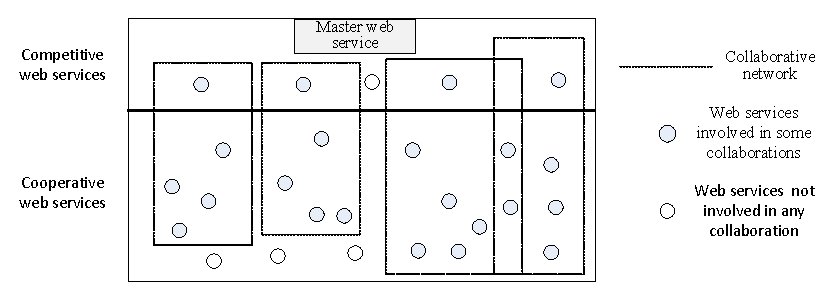
\includegraphics[scale=1]{architecture++.eps}
\caption{Services are partitioned into competitive and cooperative
sets. Competitive services may get tasks directly from the master
agent and they can share it with other cooperative services in
their collaborative networks within the same community.}
\label{architectureFigure}
\end{figure}

\subsection{Architecture}

Figure \ref{architectureFigure} illustrates the architecture of a
typical community aggregating a number of services with different
interactive strategies. Some of them compete for the task where
they directly deal with the master. Some others cooperate in the
associated task where they only deal with the competed service as
the task leader and do not directly interact with the master (the
master deals only with the service that has bid for the task,
which is responsible of choosing its collaborative network). In
both sets, some service agents are for certain moments out of any
collaboration network. Upon allocation of
the task, the service is responsible for offering the required QoS
that is stated in the task being generated by a consumer.
Afterwards,  the master rewards or penalizes the competing
service by upgrading or degrading its reputation according to the
offered QoS compared with the required one. This comparison
influences the sorting mechanism used by the master to allocate
the tasks in further task allocation rounds.


%ok til here


\subsection{System Parameters}
In this section, we demonstrate the involved parameters and their
corresponding formulations and explanations.

\textbf{Task QoS} ($T_{QoS}^r$) is the required QoS metric for a
specific task $r$. Users define tasks with specific QoS
requirements such as response time, availability, and
successability (or accuracy). We aggregate and
normalize these metrics to a value between $0$
and $1$. %Throughout this paper, we refer to this value as
%$T_{QoS}$.

\textbf{Service QoS} ($QoS_w^r$) is the QoS provided by the
service $w$ after performing the task $r$. Again, the metrics that
contribute in computing this QoS are aggregated and normalized to
a value between $0$ and $1$. The offered quality might or might
not meet the required task quality $T_{QoS}^r$. In the latter
case, the service user would be disappointed and a negative
satisfaction feedback is expected. In our proposed system, both
cases are considered when calculating the services' reputation.

%\textbf{NTD} is the number of tasks completed by a web service.

\textbf{Budget} ($B_w^t$) is the amount of money the service agent
$w$ has in its disposal during the window time $t$ (i.e.,
$[0,t]$), which helps pay for the community membership fees
($\epsilon$) and is one of the parameters that the service agent
considers when deciding about getting involved in a competition or
not.

\textbf{Reputation} ($Rep_w^t$) is a significant factor in any
online community \cite{Fouss:2010:PRM:1751668.1751727}. Without a reputation enabling
mechanism, users cannot differentiate among services, specially
the ones which offer the same type of service. Reputation
mechanisms usually aggregate users' experiences and in our case it
strongly depends on QoS that each service provides. Users define
tasks, each one with specific quality $T_{QoS}^r$, so that after
performing a certain number of tasks, each one with $QoS_w^r$,
during a window time $t$, the reputation of $w$ gets evaluated by
the master agent. $Rep_{w}^{t}$ refers to the reputation of $w$
during that window time $t$.

In Equation \ref{repr}, we compute the reward that the master
computes considering the task $r$'s QoS $T_{QoS}^r$ compared with
the service offered quality $QoS_w^r$. In case the offered quality
meets user expectations, the reward value would be positive. In
this system, we consider a small value as default rewards $\eta$
which the master considers together with the proportional level of
satisfaction as a weighted value (by $\upsilon$). In this case,
the higher the offered quality, the more weighted reward. In case
the offered quality did not meet the user expectations, the reward
would be negative. A default penalty value $\rho$ (where
$\rho>\eta$) together with the weighted proportional difference
are therefore considered. The idea is to harshly penalize the
services rather than rewarding them. To this end, rational service
agents should carefully analyze their capabilities once the
available tasks are announced. Equation \ref{reward} computes the
obtained reward by $w$ during the window time $t$ considering the
set $task_w^t$ of tasks performed by $w$ during the window time
$t$. In our proposal, service agents have the goal of increasing
their budget, which is directly related to their reputation. Thus,
they have to decide strategically how to maximize this value.

\begin{equation} \label{repr}
reward_w^r = \begin{cases}
\eta + \upsilon \frac{QoS_w^r}{T_{QoS}^r+QoS_w^r}   & \text{if $T_{QoS}^r\leq QoS_w^r$;}\\
-(\rho +  \upsilon \frac{T_{QoS}^r}{T_{QoS}^r+QoS_w^r} ) & \text{otherwise.}\\
\end{cases}
\end{equation}


\begin{equation} \label{reward}
reward_w^t =
\begin{cases}
\frac{\sum_{r \in
task_w^t}reward_w^r}{|task_w^t|}& \text{if $task_w^t \neq \emptyset$;}\\
0 & \text{otherwise.}\\
\end{cases}
\end{equation}

The assigned reputation value is updated by the computed reward
value. The computed reputation of services is bounded by the
minimum and maximum reputation values $0$ and $1$. % to constrain
%the balance the cooperative community of web services. The updated
%Let $\Gamma = Rep_{w}^{t} + reward_w^t$.
%The updated reputation
%value is then computed as follows:
%
%\begin{equation}\label{repz}
%%Rep_{w}^{t+1} = Rep_{w}^{t} + reward
%%\end{equation}
%%\begin{equation*}
%Rep_{w}^{t+1} = \begin{cases}
%
%\Gamma & \text{if $ 0 \leq \Gamma \leq 1$;}\\
%0  & \text{if $\Gamma < 0$;}\\
%1 & \text{if $\Gamma > 1$.}\\
%\end{cases}
%\end{equation}
%
%For new services with no previous reputation value, we use the
%bootstrapping trust technique proposed in \cite{conf/icwe/YahyaouiZ11}. This
%technique consists in giving the new services a chance and observe
%their behaviors for a period of testing time. The observation
%sequence is modeled as a hidden Markov model that is used to
%detect the behavior of the service by comparing the observation
%behavior against pre-defined trust patterns. Based on the matching
%result, an initial value is assigned to the service. Using this
%initial reputation value, services quickly converge to their
%actual and stable values using the update function.

%\begin{proposition}\label{Complexity-Rep}
%$Rep_{w}^{t}$ can be computed in time $O(|t|)$, i.e., in time
%linear in the size of the window $t$.
%\end{proposition}

%\begin{proof}\footnote{In this paper, we
%assume that the common arithmetic and elementary functions, such
%as multiplication, division and trigonometric functions can be
%computed in time $O(1)$ as they operate on inputs of fixed sizes.}
%The function $Rep_{w}^{t}$ is recursive on $t$, but the algorithm
%works by storing the last calculated reputation value in a
%variable, so it will not be recalculated again at each iteration.
%However, the calculation of $reward_w^t$ is needed. Since the
%function $reward_w^t$ can be computed in time linear in the number
%of tasks (see Equations \ref{repr} and \ref{reward}), which in
%turn is linear in the size of the window time, the result follows.
%$\Box$
%\end{proof}

\textbf{Growth Factor} ($G_w^t$) is a parameter which declares
services' performance based on their recent strategies and
activities. Growth factor is relative to services' reputation
$Rep_w^t$, QoS during the window time $t$ $QoS_w^t$, and budget
$B_w^t$. This factor is the main variable a typical service uses
to decide about which strategy to adopt. We use Equation \ref{eq:growthfactor} to compute the
growth factor $G^t_w$ of the service $w$ during the window time
$t$ as the average of the three aforementioned parameters, where
$n_t$ is the total number of offered tasks to the whole community
during the
window time $t$, %(we consider the time window $t$ large enough so
%that $n_t \neq 0$),
$\mu_w$ is the mean received service fee, and $\epsilon$ is the
cost of community membership.

\begin{equation}\label{eq:growthfactor}
G^t_w = \frac{Rep^t_w + QoS_w^t+\frac{B_w^t}{n_t  \mu_w -
\epsilon}}{3}
\end{equation}
\begin{equation*}
\mu_{w} \in\{\mu_{w, CM}, \mu_{w, CO}\},~~~QoS_w^t =
\begin{cases} \frac{\sum_{r \in
task_w^t}QoS_w^r}{|task_w^t|}& \text{if $task_w^t \neq \emptyset$;}\\
0 & \text{otherwise.}\\
\end{cases}
\end{equation*}


  % if the profit $\beta_w$ made by the web service $w$
%considering the mean received service fee $\mu_w$ and the cost of
%community membership $\epsilon$ is positive.
%It is easy to show that Equation \ref{eq:growthfactor} satisfies
%the three aforementioned properties by calculating the partial
%derivatives $\partial G^t_w$ of this function in 1) $QoS_w^t$
%($\frac{\partial G^t_w}{\partial QoS_w^t} = \frac{1}{3} $); 2)
%$Rep^t_w$ ($\frac{\partial G^t_w}{\partial Rep^t_w} = \frac{1}{3}
%$); and 3) $B_w^t$ ($\frac{\partial G^t_w}{\partial B_w^t} =
%\frac{1}{3 (n_t \mu_w - \epsilon)} $). Thus, the sign of the two
%first partial derivatives is positive and the sign of
%$\frac{\partial G^t_w}{\partial B_w^t}$ depends on the sign of the
%maximum profit $n_t \mu_w - \epsilon$, so we are done.
The mean
service fee depends on the strategy adopted by the service because
a competitive service receives higher fees $\mu_{w, CM}$ compared
to a cooperative one $\mu_{w, CO}$ ($\mu_{w, CM} > \mu_{w, CO}$).
The motivation behind this is that a competitive service for a
given task is the leader for that task while other cooperative
services are performing specific subtasks as asked by the leader.


%\begin{proposition}\label{Complexity-Growth_Factor}
%$G_w^t$ can be computed in time linear in the size of the window
%$t$.
%\end{proposition}
%
%\begin{proof}
%As shown in the second part of Equation \ref{eq:growthfactor}, the
%function $QoS_w^t$ can be computed in time linear in the number of
%tasks, which in turn is linear in the size of the window time.
%Since $B_w^t$ is constant, the result follows from Proposition
%\ref{Complexity-Rep}. $\Box$
%\end{proof}


\subsection{Service Interactive Strategies}

The main goal of each individual service agent is to increase its
income (payoff). This income can be earned from tasks (or
requests) done by this service. In our model, services can decide
to compete to get a task from the master agent or to cooperate
with other services within a given collaborative network (the way
a collaborative network is set by a leader is based on the
cooperative services reputation and their QoS parameters that
should coincide with the required QoS). Therefore we define two
types of service strategies. First, when a service has higher
level of confidence based on its growth factor, it can compete to
get a task from the master and adopts the competitive strategy.
Second, when the service agent has a lower level of confidence
that it does not feel capable to compete, it waits for some other
services to cooperate with to perform some tasks \footnote{Through
the report, requests or tasks are supposed to be decomposable.},
and thus it adopts the cooperative strategy. Services estimate the
outcome of all the strategies and choose one of them accordingly.
This decision is not static but can change over time so service
agents can switch from one strategy to the other, and this dynamic
attitude is referred to as coopetition.







\section{Experimental Results and Analysis}\label{s:resutls}

\subsection{Coalition Formation and Stability}

In this section, we discuss the experiments we performed for our
scenarios to validate the applicability and performance of our
proposed methods in realistic environments.
An XML SOAP based messaging system was implemented. The request
contains the flight dates, the origin and destination, type of
tickets, and number of guests. The response contains different
flights with different companies, prices, timing, etc. We have
gathered around 200,000 flights and stored them in our MongoDB
database. We created a pool of web services and populated most of
their \emph{QoS} parameters from a real world web service dataset
\cite{DBLP:conf/smc/Al-MasriM09a}\footnote[1]{The implemented
environment includes the QWS dataset by Eyhab Al-Masri and Qusay
H. Mahmoud freely available at:
http://www.uoguelph.ca/\textasciitilde{}qmahmoud/qws/.}. To test
our methods, we formed around 10,000 random coalitions consisting
of 3 to 160 web services. In average, the communities were populated by 60 web
services. We implemented the
scenarios using Java and executed the experiments on an Intel Xeon
X3450 machine with 6GBs of memory.

One of the key criteria reflecting the performance of web service
coalitions is the user satisfaction. User satisfaction can be
measured in terms of quality and quantity of requests (or tasks)
successfully answered by the communities. We initiate the
communities with few web services, then let rejecting and
accepting random web services go for a short number of iterations.
After that, we start the request distribution for the communities
and let them allocate requests among member web services.
Thereafter, we measure the average output performance of tasks in
communities following different methods.

\begin{figure*}%[!t]
\centering
%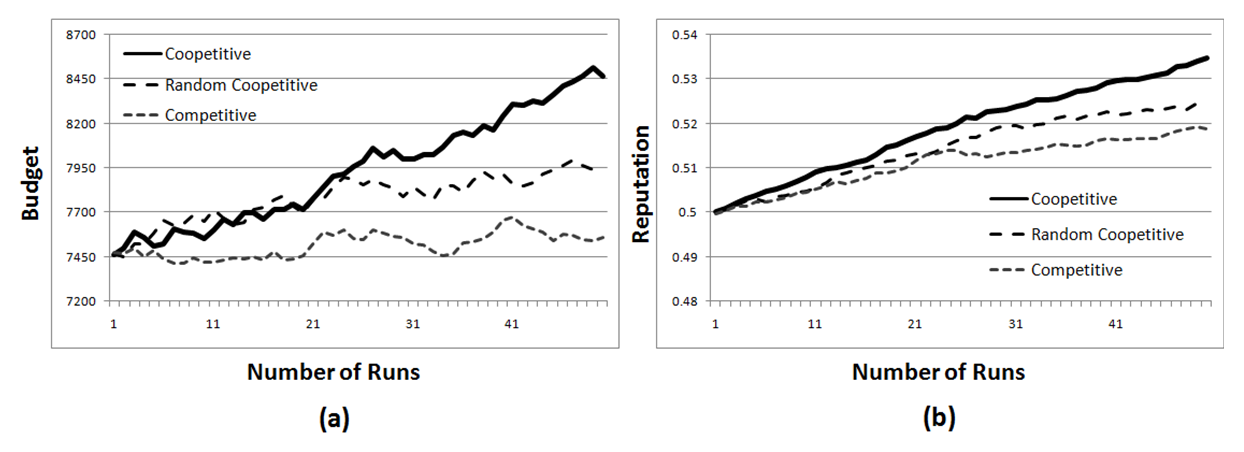
\includegraphics[scale=0.6]{graph1Final+.eps}
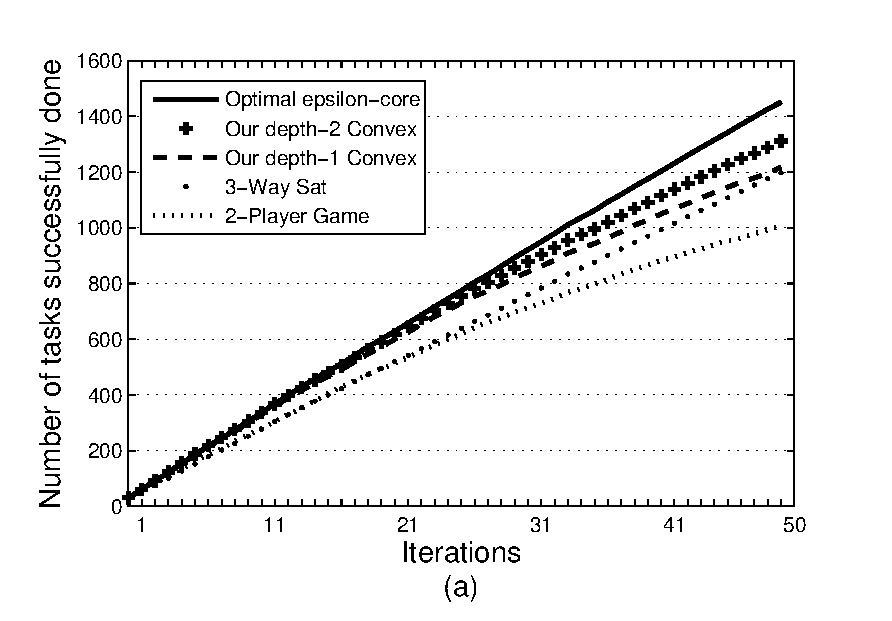
\includegraphics[width=2.8in]{task_done_opt.eps}
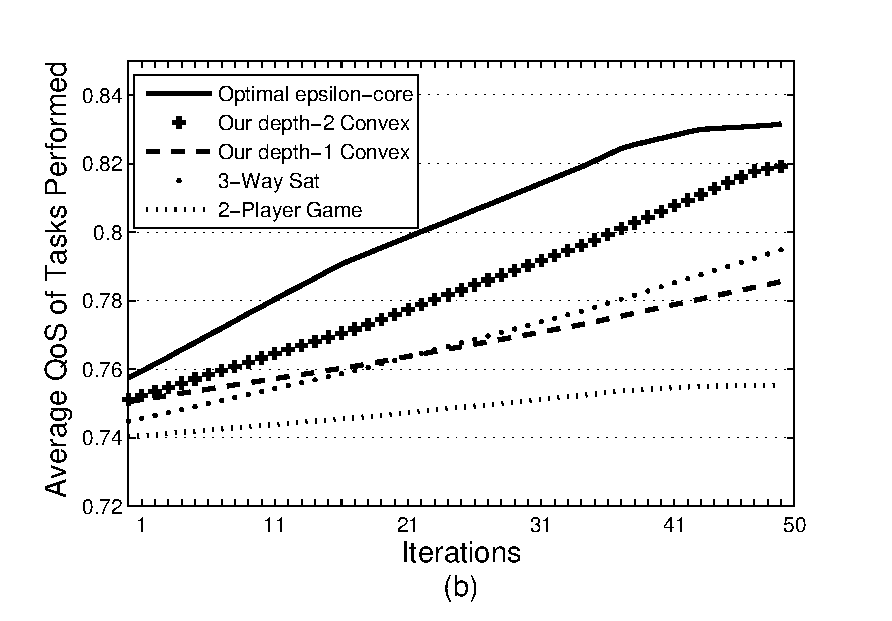
\includegraphics[width=2.8in]{task_qos_opt.eps}
\caption{Part (a): Cumulative number of requests successfully
done. Part (b): Average QoS of requests performed.}
\label{performanceall}
\end{figure*}

Figure \ref{performanceall} depicts the results of our methods:
\emph{Depth-1 Convex-Checker} and \emph{Depth-2 Convex-Checker},
and compares them with \emph{3-Way Satisfaction} (from
\cite{DBLP:conf/IEEEscc/LimTMB12}), and \emph{2 Player
Non-Cooperative} (from \cite{DBLP:conf/IEEEscc/KhosravifarABT11})
methods in \emph{one grand community with many web services}
scenario. The figure also depicts the results of the theoretical
\emph{optimal $\epsilon$-core} as benchmark.


For the \emph{optimal core} method, we have used the well known
\emph{$\epsilon$-core} method as the taxation method to relax the
core condition to help communities attract web services. We have
assigned $\epsilon$ to 15\% of total community worth, which means
$\epsilon = 0.15 \times v(C)$. This allows subsets of the
coalition to gain maximum 15\% of $v(C)$.
%In the \emph{optimal
%$\epsilon$-core} method, we capped the coalition size to 25 web
%services, since the method is computationally intractable as the
%number of web services increases. In fact, given the machine
%configuration we used in our experiments, the maximum number we
%could run for this method is 25, which is very realistic if we
%consider the real airlines coalitions (the three well known
%coalitions have respectively 28, 19, and 13 members). In the other
%methods, there were no cap on size of the community and we had
%communities of size 160 web services at some points, as discussed
%above.
In the experiments, our \emph{Depth-1 Convex-Checker} and
\emph{Depth-2 Convex-Checker} methods generate results instantly
(0.01ms in Java millisecond time unit granularity) in our machines
since their runtime with respect to the size of input (number of
web services) is $O(n)$ and $O(n^2)$ respectively. This shows that
the algorithms are efficient and the system is easily scalable. In
this scenario, our community receives 130 tasks from users on
average per iteration. These tasks are randomly generated.
%These tasks are about flight booking and
%are expected to be performed by the community. They are randomly
%generated using a poisson distribution (having 130 as parameter).
Depending on community task queue and the assigned web services'
quality metrics the task will be performed with some qualities.
The community, after the task distribution process on each
iteration, will reevaluate QoS metrics of its members and can
check for new membership requests. Web services may join or leave
the community between iterations. The results show that our
\emph{depth-2 convex checker} method is performing better compared
to the other methods and its performance is close to the optimal
\emph{$\epsilon$-core} method. Our \emph{depth-1 convex checker}
and the \emph{3-Way Satisfaction} method, are also performing
well.

%
%\begin{figure*}%[!t]
%\centering
%%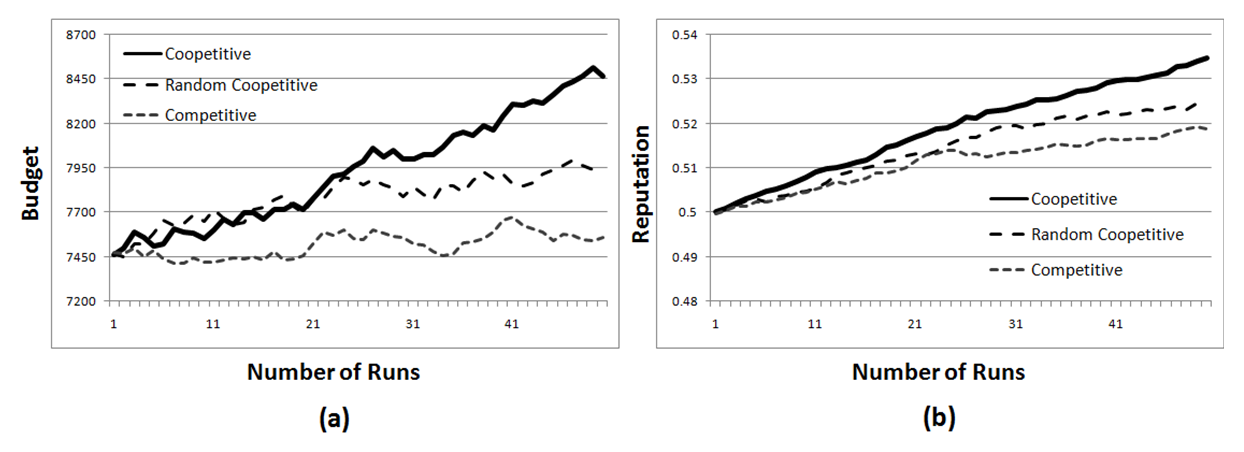
\includegraphics[scale=0.6]{graph1Final+.eps}
%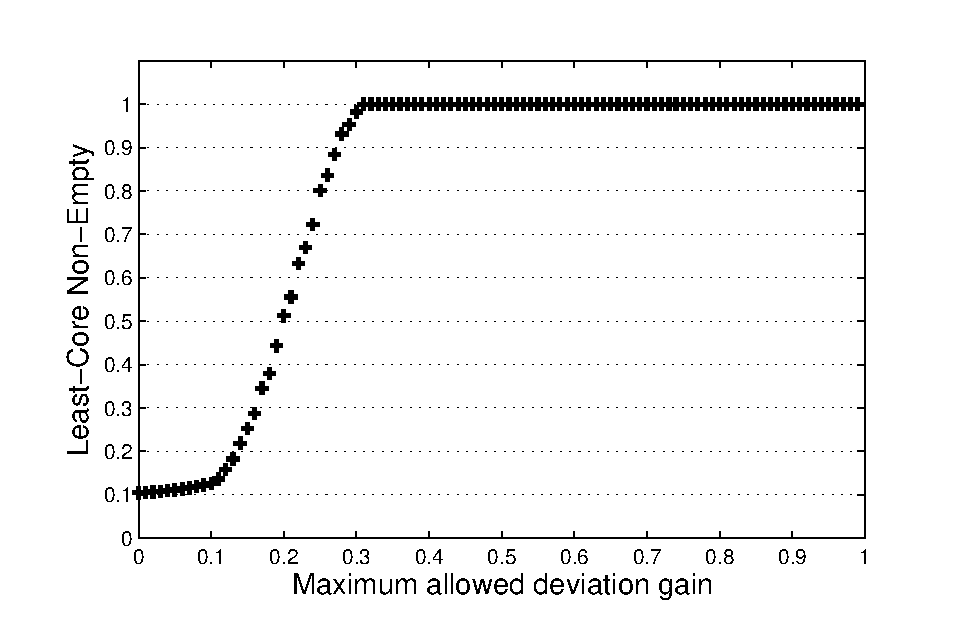
\includegraphics[width=3in]{least_core.eps}
%\caption{Analysis of \emph{$\epsilon$-core} set non-emptiness for
%different values of $\epsilon$} \label{f_leastcore}
%\end{figure*}
%
%As mentioned in Section \ref{s:preliminaries}, the concept of
%\emph{core}, assumes no coalition of players can gain anything by
%deviating, which is a fairly strong requirement, and that is why
%the notion of \emph{$\epsilon$-core} was introduced. Least-Core
%$e(G)$ of a game $G$ is the minimum amount of $\epsilon$ so that
%the core is not empty. We evaluated the non-emptiness of
%\emph{$\epsilon$-core} set using our valuation function and a set
%of web services from our coalitions.  The restriction on the
%number of web services per coalition for this particular method is
%justified because it is
%very complex for larger coalitions to verify whether
%\emph{$\epsilon$-core} set is empty or not. Also instead of
%considering $\epsilon$ amount of constant deviation in
%\emph{$\epsilon$-core} definition (Equation \ref{eq:core2}), we    %TODO FIX THIS
%similarly defined \emph{relative $\epsilon$-core} concept where no
%coalition would benefit more than \emph{$\epsilon \times v(C)$} by
%deviating. We vary $\epsilon$ so that it takes different values
%from $0$ to $1$ and observe the impact in terms of verifying the
%\emph{relative $\epsilon$-core} set non-emptiness. The results in
%Figure \ref{f_leastcore} illustrate that almost 10\% of our random
%web service coalitions have non-empty \emph{core} solution and
%\emph{$\epsilon$-core} solution is \emph{always} non-empty when we
%let agents gain only 30\% more of $v(C)$ by deviating.


\begin{figure*}%[!t]
\centering
%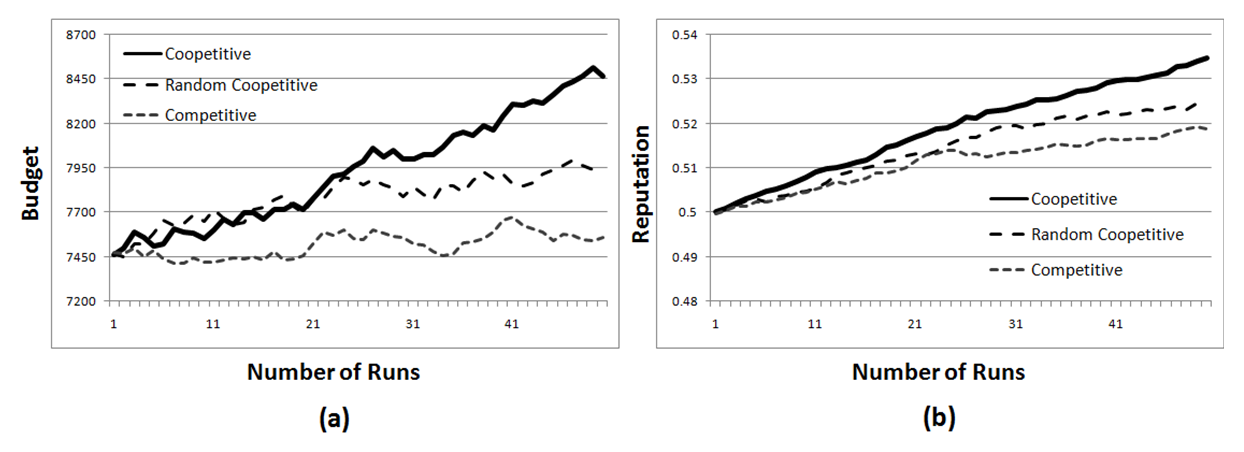
\includegraphics[scale=0.6]{graph1Final+.eps}
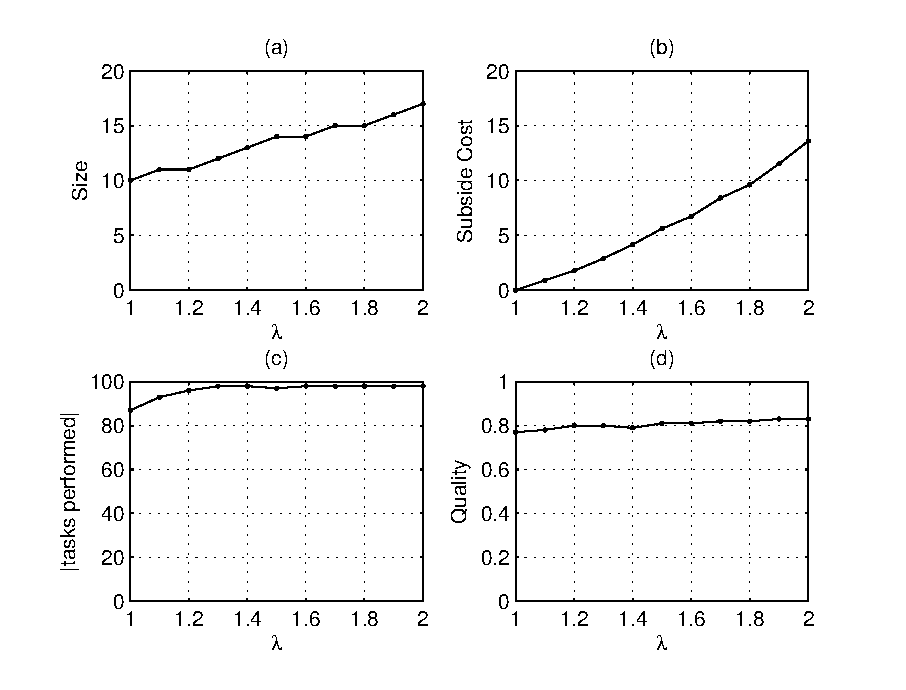
\includegraphics[width=3in]{taxtation.eps}
\caption{Analysis of community subsiding coefficient $\lambda$ on
average community size (a), cost (b), number of tasks performed
(c), and average quality of service of tasks performed (d).}
\label{f_taxtation}
\end{figure*}

As mentioned in Section \ref{s:tax}, a solution to help the
community stabilize is to subside the community by a relative
coefficient ($\lambda$) so the value of $\lambda v(C)$ is divided
among the community members. We have analyzed the effect of
subsiding and the cost it incurs to our web service communities.
Figure \ref{f_taxtation} shows the results. In this experiment, we
have set a community with input task rate $R_C$ of 100 and having
web services throughput rate $Th_{ws}$ values from a normal
distribution with average 10 tasks per iteration and standard
deviation 2. Part (a) shows the community size increases in a
linear fashion as ($\lambda$) increases. However, the cost (Part
(b)) is having a slight exponential growth rate since, not only
($\lambda$) increases, but also the size of the community is
increasing slowly. Therefore, subsiding can be costly for larger
number of $\lambda$ values. Part (c) depicts the number of tasks
done by the community per iteration. It is obvious that with
$\lambda$ value of 1.3, which is 30\% of the community valuation,
the number of tasks done almost reaches the input task rate cap of
100 tasks per iteration. The average quality of tasks also has a
slight increase since the community will be able to afford better
and more web services to join the community (Part (d)). These
results show the effectiveness of our subsiding method and its
impact on the QoS. In fact, using more than 30\% of the community
valuation as subsidy is not very effective and is costly to
perform.

\begin{figure*}%[!t]In the previous experiment, we considered the scenario where all
web services are stable, will not leave the group, and will
fulfill their promised QoS for a good period of time. However, in
real world scenarios of web services, this is not always the case.
This is the reason why the community coordinator would be interested in paying
web services in order to keep the group reliable from the end
user's point of view.
\centerline{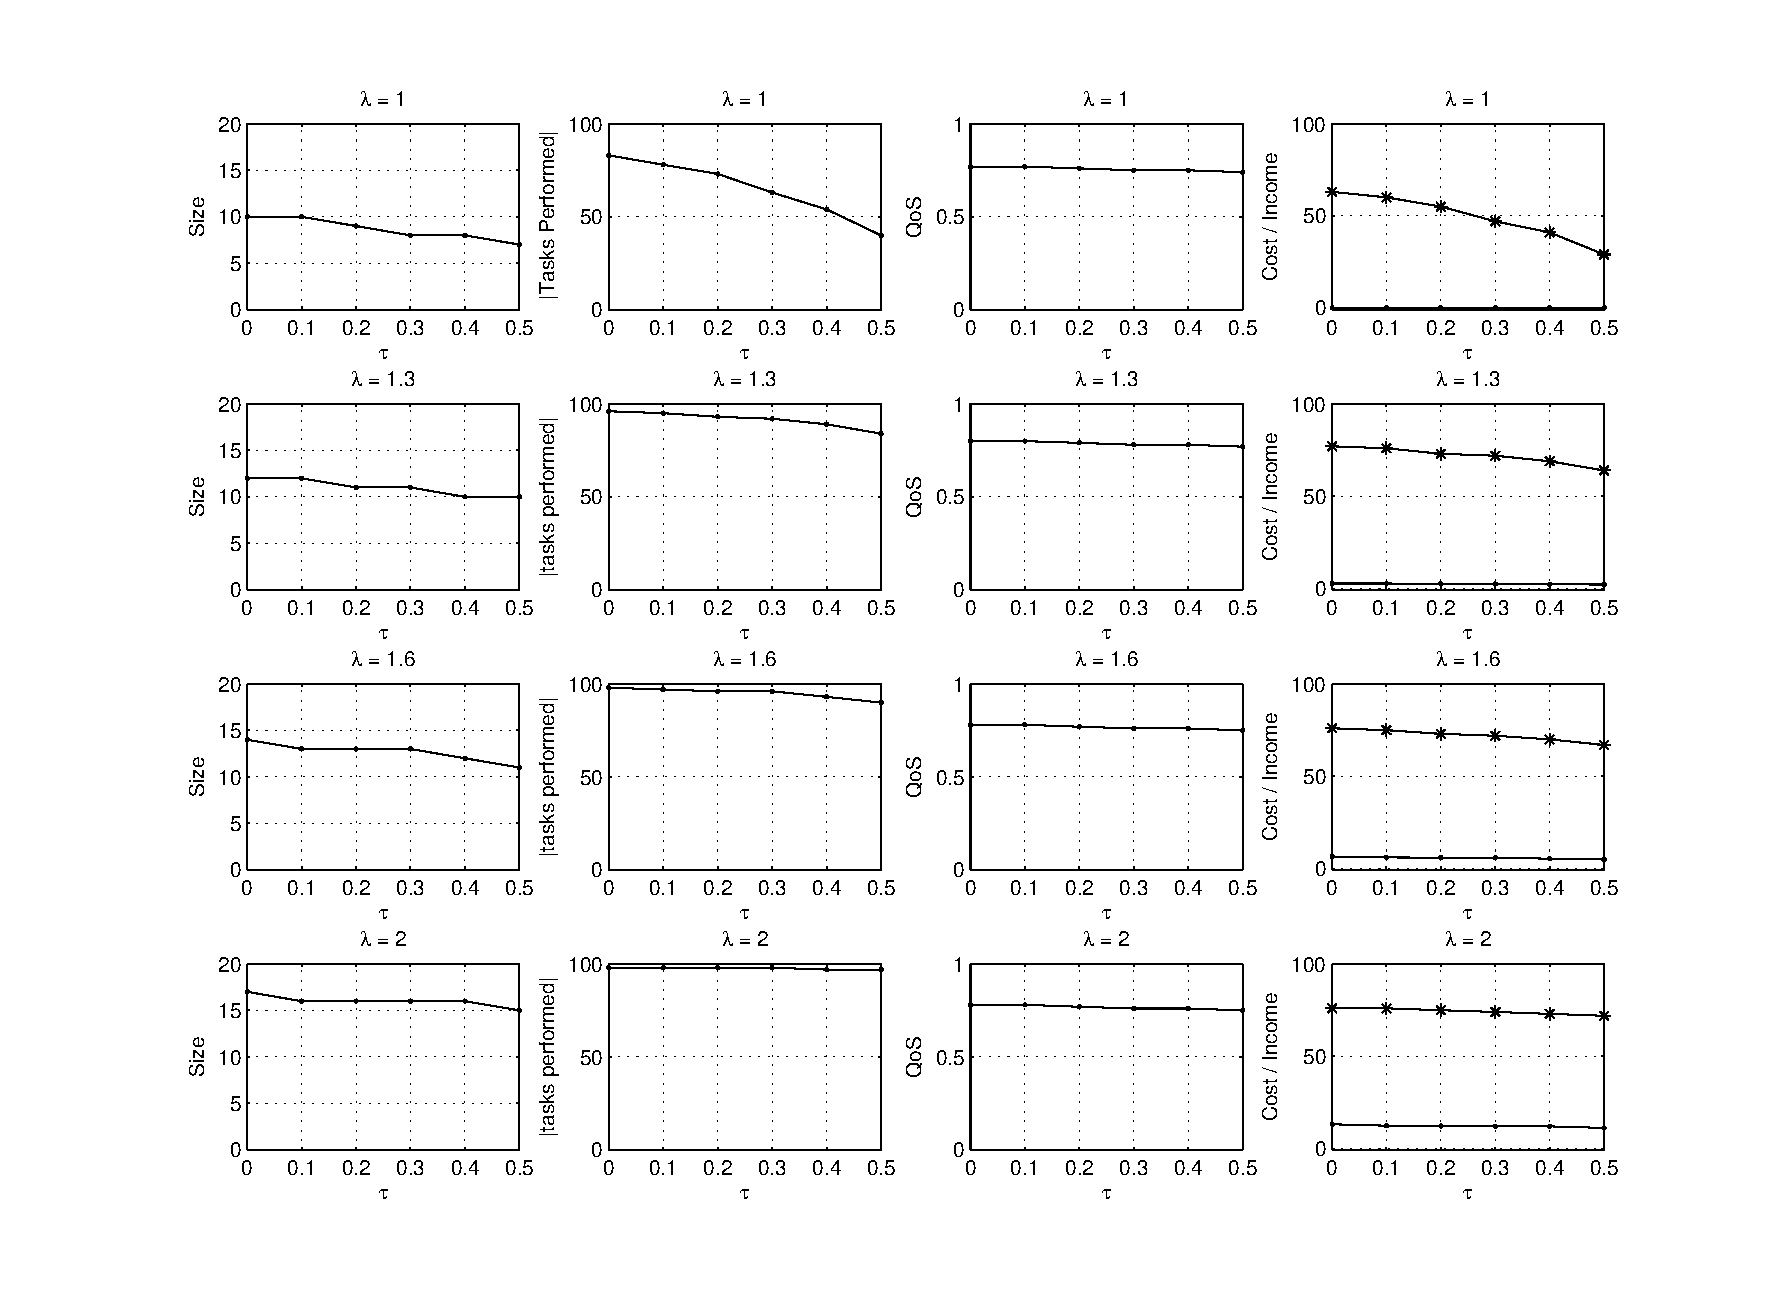
\includegraphics[width=6.8in]{tax_dyn.eps}}
\caption{Analysis of community subsiding coefficient $\lambda$
having web service different stability levels of $\tau$ on average
community size, number of tasks performed, average quality of
service, and average cost/income of communities.}
\label{fig_dynamic_taxtation}
\end{figure*}


In our next scenario, we have introduced the
new instability variable $\tau$ ranging from 0 to 1, 0 meaning web
services having no instability issues and will perform as they
claimed until the end of the experiment, and 1 meaning very
unstable web services, which will stop functioning on the first
iteration of the community distributing tasks. Figure
\ref{fig_dynamic_taxtation} illustrates the results of our
experiment having web services with average instability values of
0 to 0.5 and having relative subside value $\lambda$ of 1, 1.3,
1.6, and 2. The \emph{Cost/Income} charts on the right column show
that having subside value of 1.3 incurs the least cost and
increases the community income significantly. Subsiding values of
1.6 and 2 yield high cost to the community and only slightly
increase the community revenue. Moreover, the role of subsiding is
much more obvious when we have unstable web services. In scenarios
where web services are 100\% stable, the subsiding cost will
hardly be compensated by the community revenue.

\begin{figure*}%[!t]
\centering
%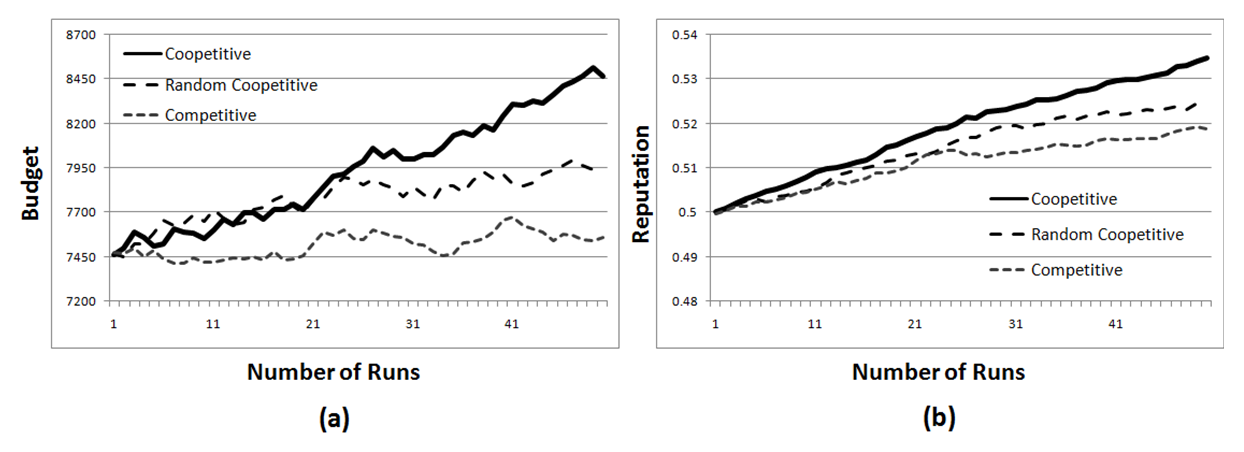
\includegraphics[scale=0.6]{graph1Final+.eps}
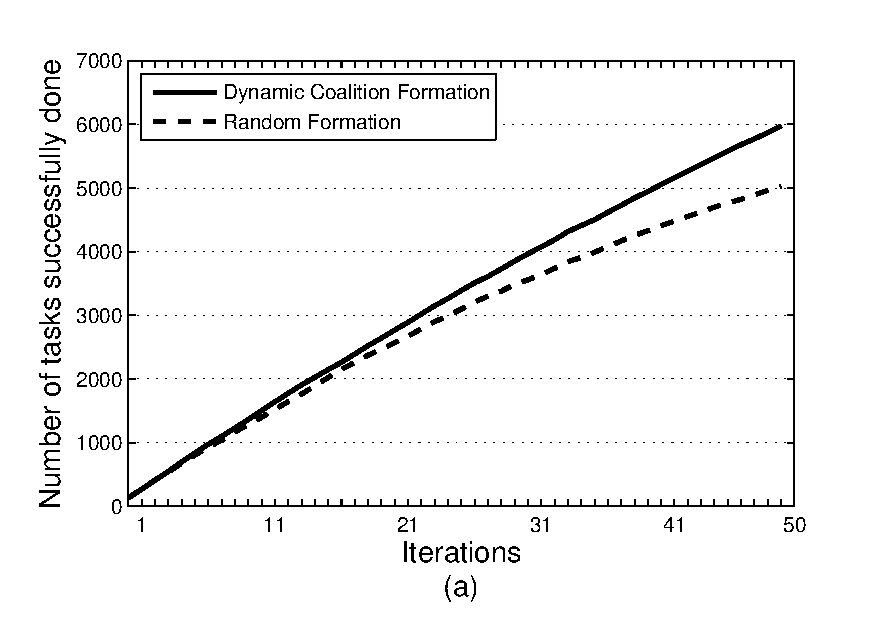
\includegraphics[width=2.8in]{s2_task_done.eps}
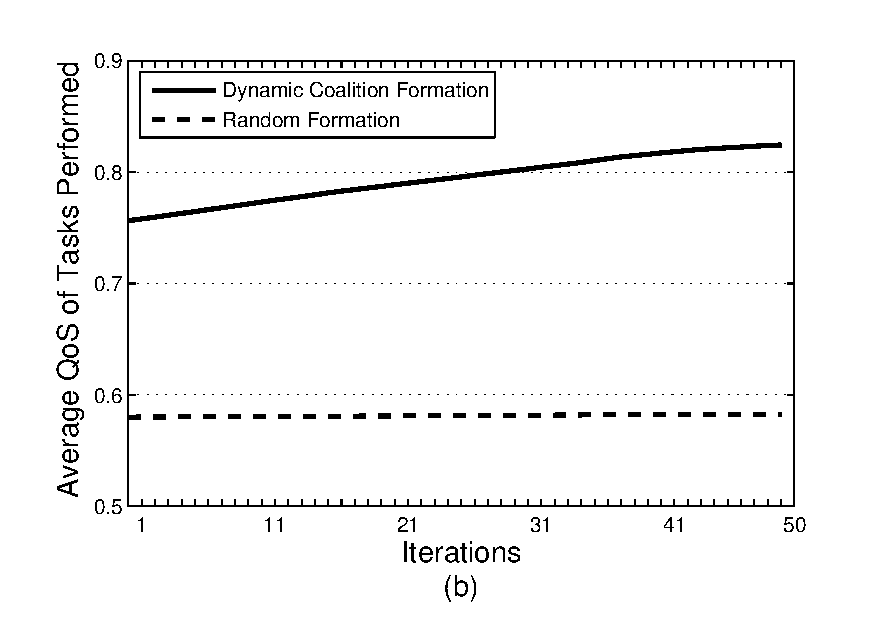
\includegraphics[width=2.8in]{s2_task_qos.eps}
\caption{Part (a): Cumulative number of tasks successfully done.
Part (b): Average QoS of tasks performed.} \label{performancemany}
\end{figure*}


In Figure \ref{performancemany}, we consider \emph{Web Services
and many Communities} scenario and we compare our dynamic
coalition formation solution with a method which ignores QoS
parameters and forms communities by allowing web services to join
only if they have enough requests for themselves. In other words,
web services can join a community when the request rate is less
than the throughput of all the member web services. We name this
method \emph{Random Formation} and use it as a benchmark for our
QoS-aware community formation process. In this scenario, each user
individually generates randomly between 0 to 10 number of tasks
per iteration, then the users target a community and direct their
requests to the chosen community. As the results illustrate, our
method forms better communities of web services improving
performance and satisfaction for both web services and
communities.

\begin{figure*}%[!t]
\centering
%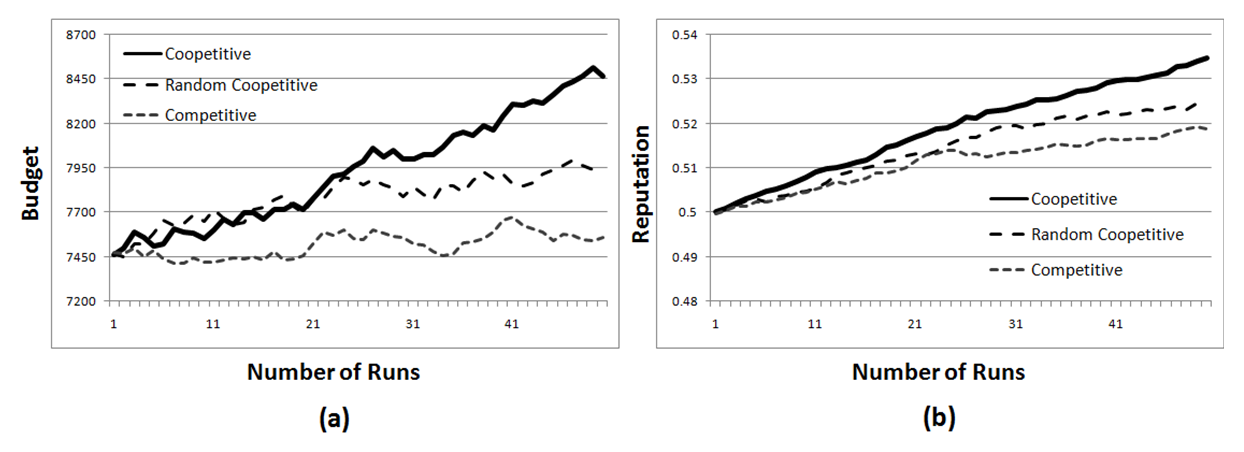
\includegraphics[scale=0.6]{graph1Final+.eps}
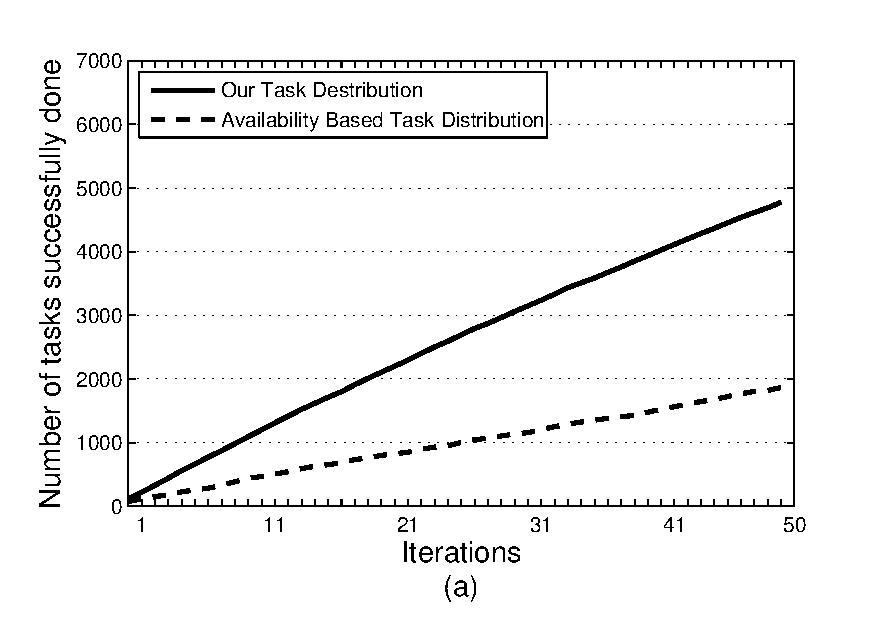
\includegraphics[width=1.9in]{avg_task_ws_done.eps}
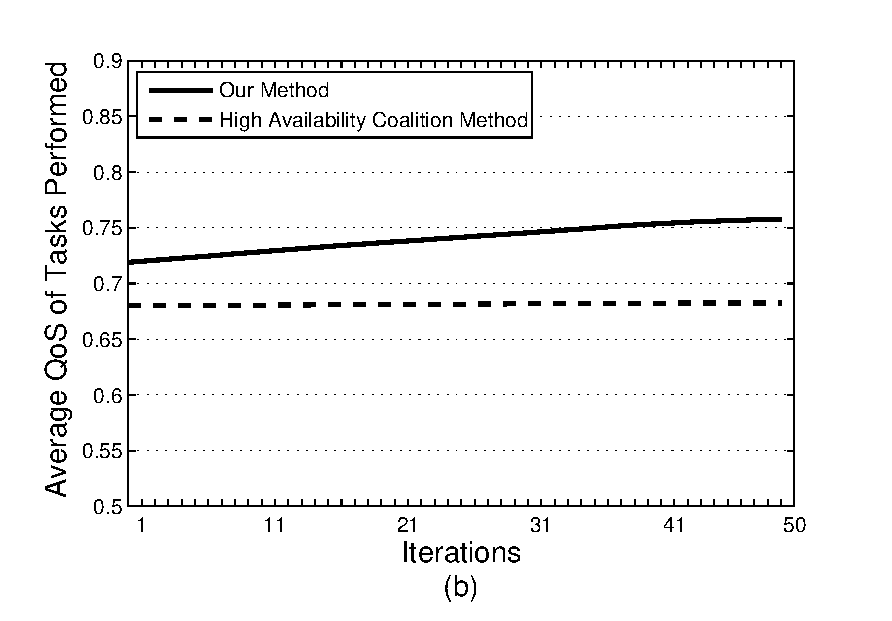
\includegraphics[width=1.9in]{avg_qos_ws_done.eps}
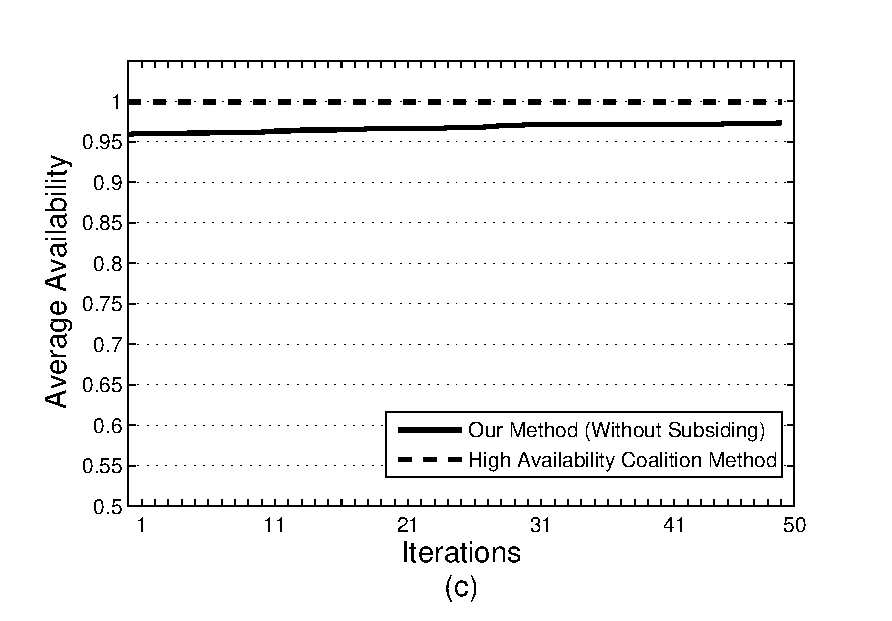
\includegraphics[width=1.9in]{avg_avail_ws_done.eps}
\caption{A comparison between our community model and the High
Availability Coalition model from \cite{10.1109/TSC.2012.12}. Part
(a): Cumulative number of tasks successfully done. Part (b):
Average QoS of tasks performed. Part (c): Average community
service availability} \label{fig_avail_method}
\end{figure*}

Finally, in our last experiment, we compare our model with the
solution proposed in \cite{10.1109/TSC.2012.12}, which we call
\emph{High Availability Coalition} model. In this method, the
community valuation function focuses on the community availability
as main consideration. The community formation model used in this
method is very different from ours, but we have been very careful
to make the experiment environment as fair and similar to ours as
possible. We limited our maximum community size to 5 in order to
have communities with almost the same size as in
\cite{10.1109/TSC.2012.12}. In the High Availability Coalition
model, the authors have used web services as backups rather than
active collaborative players, and those web services only get a
task when the first web service in an ordered chain fails to
perform that task. %However, with recent advancement in cloud and
%hardware infrastructures, availability is less of an issue for web
%services, and web services are highly available.
Part(a) of Figure \ref{fig_avail_method} shows that with our
method, the number of tasks successfully done is higher with a
rate of three times more than the High Availability Coalition
model thanks to the cooperative behavior of web services and the
task distribution process of our algorithm. This result shows that
using web services as backups, and not as real collaborative
players results in a considerable waste of web services capability
since services have very low chance of getting jobs and its the
primary web service (the first in the coordination chain) which
does most of the work. As shown in Part (b), the average quality
of service of tasks performed using our solution is also higher
since our method considers all quality of service metrics used. Part(c) shows the availability of
communities from the end user's point of view. The High
Availability Coalition model has almost 100\% uptime since web
services are used as backups, so the chance of job failing is
getting reduced significantly as community members increase. In
our method, we have more chance of failure for each web service.
However, with some subsidies and by hiring a few more web
services, the chance of failure of web services in our communities
can be lowered.

\subsection{Coopetitive Behavior}\label{sb:resutlscoop}

In this section, the objective is to investigate the effectiveness of the proposed strategic system in Section \ref{s:coop}.
We start our discussions with cumulative budget comparison
regarding different communities within which services follow
different reasoning techniques. Figure \ref{Graph1} part (a)
illustrates three graphs for three different communities. Each
community hosts services that follow different reasoning
techniques: (1) a community that follows the interactive reasoning
techniques presented in this report (referred to as coopetitive);
(2) a community that follows a stochastic reasoning technique so
decisions about selecting competitive or cooperative strategies
are totally random (referred to as random coopetitive); and (3) a
competitive community where all services follow the competitive
strategy (referred to as competitive).
%The proposed model's
%reasoning mechanism allows services to make decisions that
%maximize their utilities, so that if the service cannot compete,
%the procedure would suggest to collaborate, which is better than
%competing and failing to obtain the task. In this case, the service stays idle but
%still pays the community membership fee, which means losing
%utility. The developed strategic decision making mechanism leads
%some service agents to follow cooperative strategies that overall
%maintain an optimal community budget. In the same figure, we
%observe the cumulative budget of a community where services follow
%random interacting strategies. The outcome is clearly lower
%because services at each run randomly decide over their acting
%strategies. This potentially influences the community budget
%because a low quality service if randomly selects to follow the
%competitive strategy, it will fail to perform a task with high QoS
%requirements.


The results illustrated in Figure \ref{Graph1} part (a)  verify
the importance of the strategic decision making procedure to
logically decide over the possible competitive and cooperative
choices. Figure \ref{Graph1} part (b) illustrates communities
average reputation of involved services. The graphs represent the
influence of the rewards that the master agent uses to encourage
highly capable services to compete for a task. As for the
cumulative budget, we observe that the coopetitive community
outperforms the random coopetitive and competitive communities in
terms of average reputation. The proposed model's average
reputation increases because services follow optimal strategies
where they can perform better so obtain higher rewards. For the
same reasons as for the cumulative budget, the average reputation
of the random coopetitive community
outperforms the one of the competitive community. %The idea is to balance web
%services' strategies to maintain optimal community budget.


\begin{figure}%[h]
%\centering
%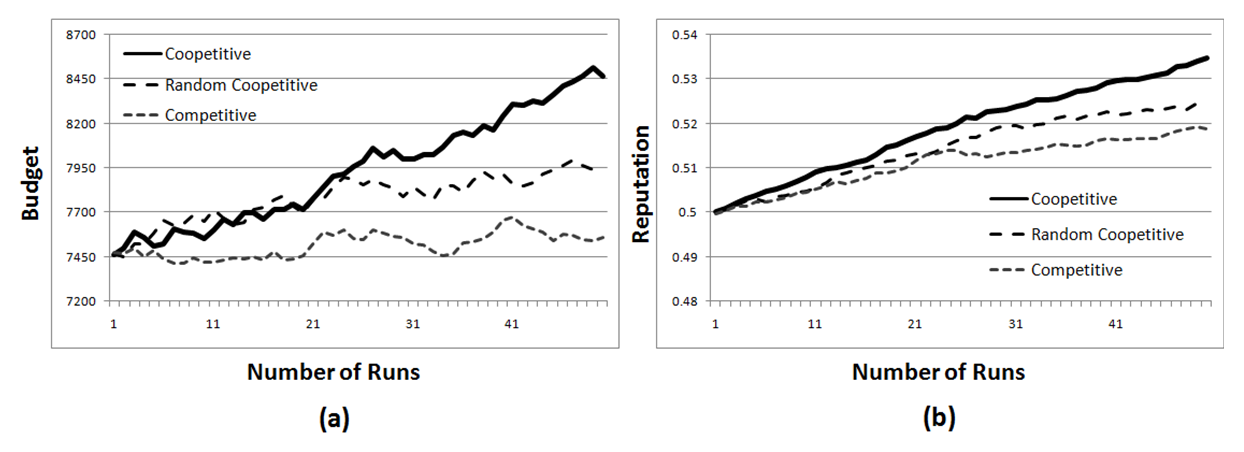
\includegraphics[scale=0.6]{graph1Final+.eps}
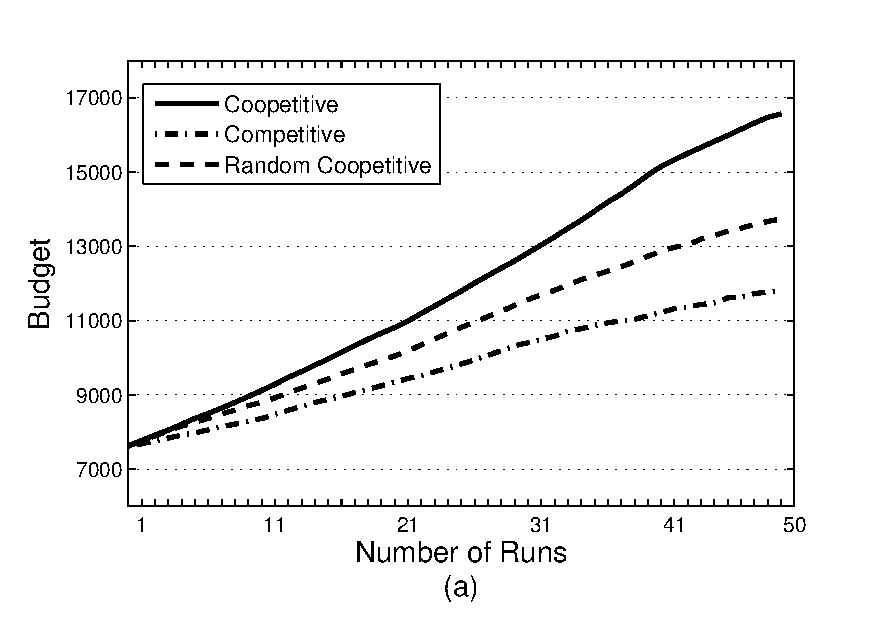
\includegraphics[scale=0.47]{graphbgtmed.eps}
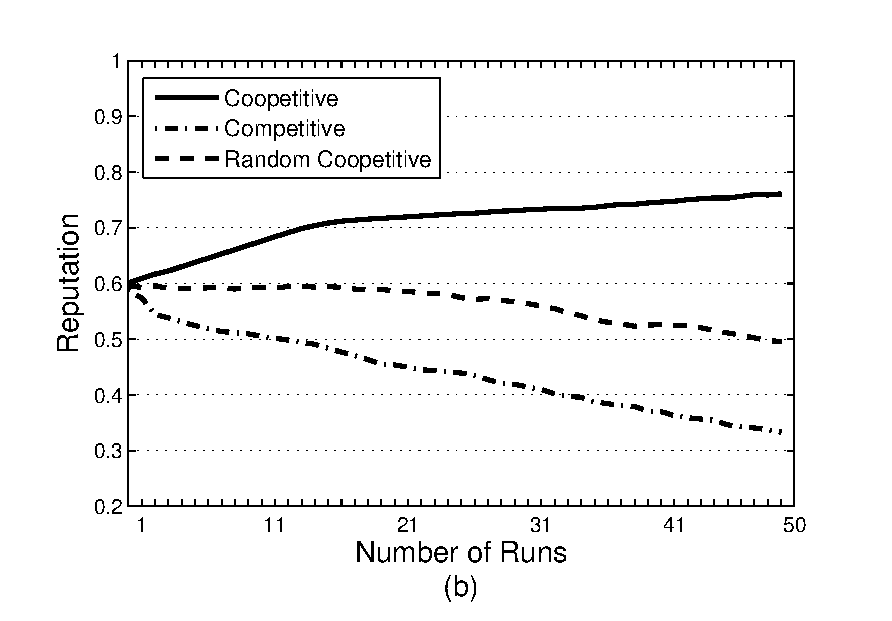
\includegraphics[scale=0.47]{graphrep.eps}
\caption{Part (a): Cumulative community budget comparison. Part
(b): Average community reputation comparison over different
strategic decisions.} \label{Graph1}
\end{figure}



 %Figure \ref{Graph2} part (a) illustrates the reputation of the proposed $Coopetitive$ community where
 %we highlight the range of reputation change in the community. The vertical lines denote the range of %reputation that is associated with the master web service. The rewards and penalties applied to %different
% web services show that the master web service over runs extends the reputation range and takes %control of the whole community. In the developed model, web services are encouraged to choose
 %optimal strategies. This is maintained over growth factor comparison of the $Coopetitive$ web %services.


In our model, services are managed by selfish agents in the sense
they try to maximize their own utilities. We analyze how their
strategies affect the social welfare, and from user's and
community's point of view how good the tasks are being performed.
This directly impacts user's satisfaction and community's
reputation in general. The Higher quality and quantity of tasks
performed leads to higher user's satisfaction for the community
which results in better reputation for the community. The results
in Figure \ref{graph_task} show the quality and quantity of tasks
being done successfully in three communities adopting the three
different aforementioned strategy decision algorithms. As clearly confirmed by the simulation, the coopetitive community
outperforms the stochastic and compete communities.

\begin{figure}[h]
\centering
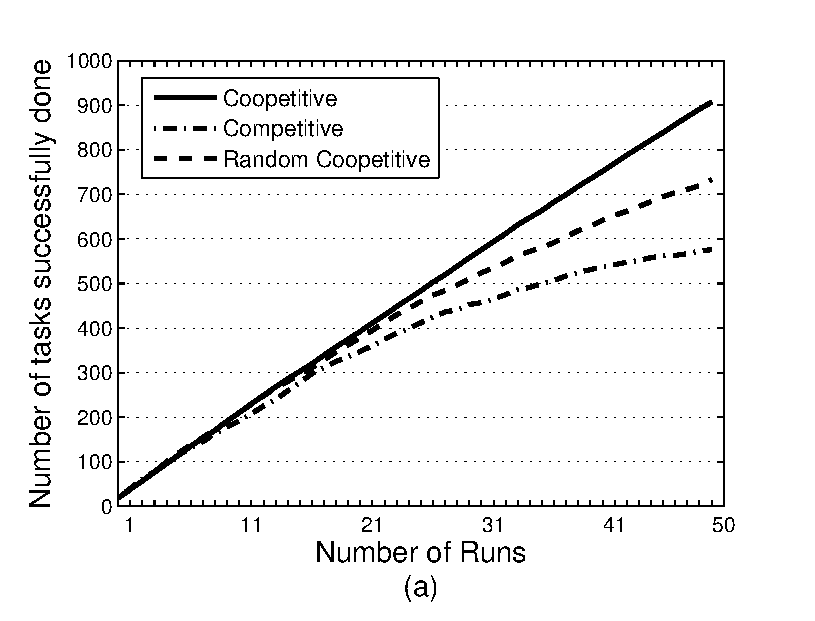
\includegraphics[scale=0.35]{graphtaskdone.eps}
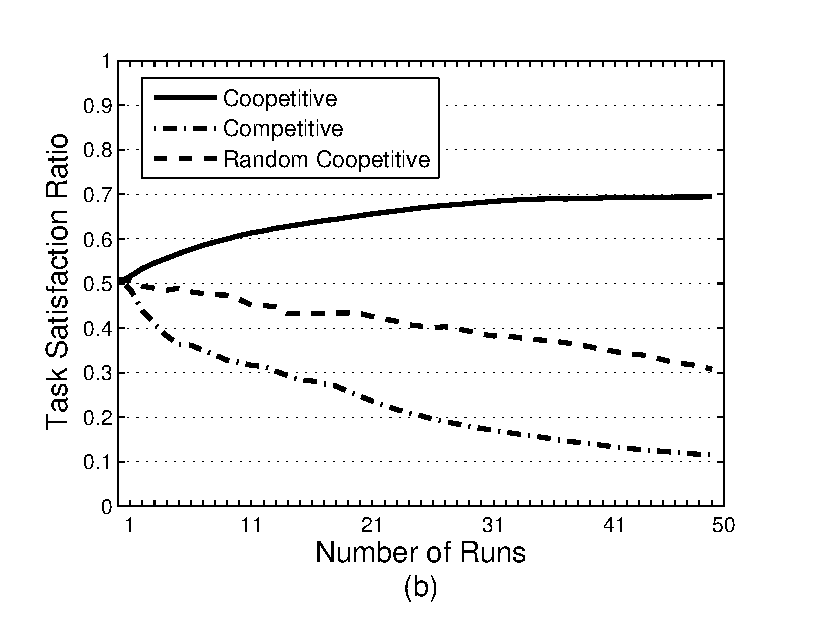
\includegraphics[scale=0.35]{graphtasksatisfaction.eps}
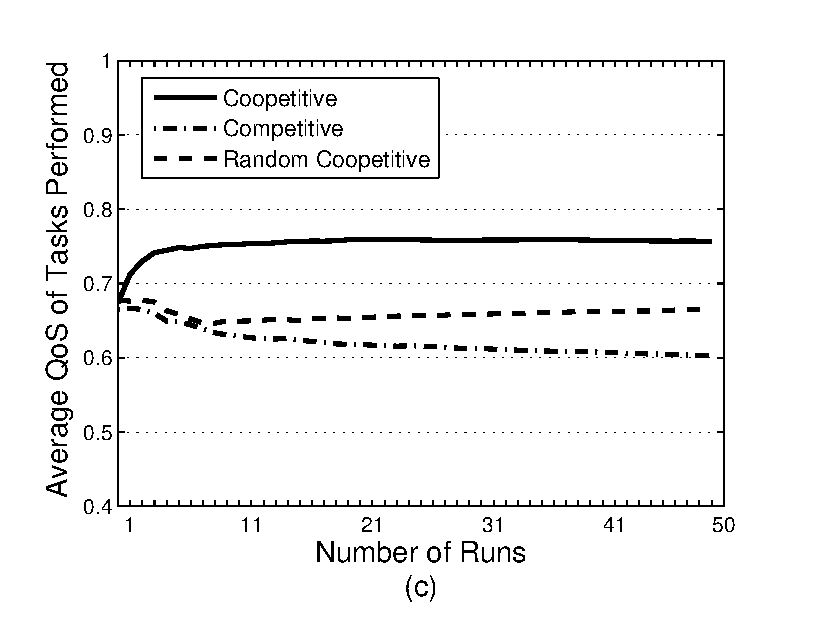
\includegraphics[scale=0.35]{graphavgqostask.eps}
\caption{Overall performance from community's point of view. Part
(a) Total number of tasks successfully done. Part (b) Ratio of
tasks satisfied with required QoS. Part (c) Average QoS of
performed tasks.} \label{graph_task}
\end{figure}

